\documentclass[a4paper,11pt]{scrartcl}
\usepackage{../packages/geosoftware}
\begin{document}
\title{Geosoftware II \\ \small Handbuch}
\author{Arndt, Autermann, Demuth, Fendrich, Ottenhues, Paluschek}
\date{\today}
\version{1.0}
\status{Entwurf}
\authormail{sloth@vespuccis.de}
\maketitle
\thispagestyle{empty}
\begin{center}
\bf Vers.: \MyVersion \\
\bf Stadium: \MyStatus\\
\bf Seiten: \thelastpage \\
\bf Kontakt: \email \\
\end{center}
\newpage
\tableofcontents
\newpage



\section{sloth.city}
Auf der Internetseite von sloth.city ist es Bewohnern der Stadt Münster möglich Beschwerden einzureichen. Von zu Hause aus lassen sich Beobachtungen wie Schlaglöcher, Müll und Vandalismus eintragen. Die zuständige Abteilung der Stadt Münster wird diese dann bearbeiten und hoffentlich zu ihrer Zufriedenheit lösen.

In diesem Handbuch werden die Möglichkeiten beschrieben, um ein erfolgreiches interagieren zwischen Administrator, Benutzer und Webseite, zu gewährleisten. Es soll helfen Probleme mit der Seite sloth.city zu lösen. Durch Screenshots wird versucht den beschreibenden Text visuell zu unterstützen, was hoffentlich zu einer besseren Problembewältigung fährt.

Auf der Seite sloth.city wird es 3 Arten von Benutzern geben. Auf der einen Seite den Administrator, dem mehr Rechte zugesprochen werden, als dem "`normalen"' Nutzer. Der "`normale"' Nutzer verfügt somit über eingeschränktere Möglichkeiten, die später noch erläutert werden. Der Besucher der Seite hat am wenigsten Rechte.


\section{Anforderungen}
Die aufgelisteten Anforderungen sollten in jedem Fall erfüllt werden, damit eine zufriedenstellende Nutzung gewährleistet werden kann.

\begin{itemize}
	\item stabile Internetverbindung (Empfehlung: DSL)
	\item Browser (Empfehlung: Mozilla Firefox 3.6, Internet Explorer 8, Google Chrome 4.1, Safari 4.0.5, Opera 10.10)
	\item Betriebssystem (Empfehlung: Windows 7, Windows Vista, Windows XP, Arch Linux \& Mac OS X 10.6.3)
\end{itemize} 

\section{Installation}
Falls sie noch keinen der obigen Browser installiert haben, sollten sie eine der aufgelisteten Seiten besuchen. Die unten genannten Seiten sind die offiziellen Seiten des jeweiligen Anbieters und sind unsere Empfehlungen.
\begin{itemize}
	\item Mozilla Firefox 3.6 \\\url{http://www.mozilla-europe.org/de/firefox/}
	\item Internet Explorer 8 \\\url{http://www.microsoft.com/germany/windows/internet-explorer/browse-with-confidence.aspx}
	\item Google Chrome 4.1 \\\url{http://www.google.com/chrome}
	\item Safari 4.0.5 \\\url{http://www.apple.com/de/safari/}
	\item Opera 10.10 \\\url{http://opera.com/}
\end{itemize} 

Sollte man Probleme bei der Installation haben, dann empfehlen wir eine Installationsanleitung. Eine Installationsanleitung für den Firefox finden sie unter dem folgenden Link: \url{http://www.firefox-browser.de/wiki/Installation}

\section{Überblick}
Im folgenden wird ein kompletter Überblick über die Seite sloth.city gegeben. Die Oberfläche wird erklärt und die einzelnen Funktionen näher erläutert.

\begin{figure}[h]
\centering
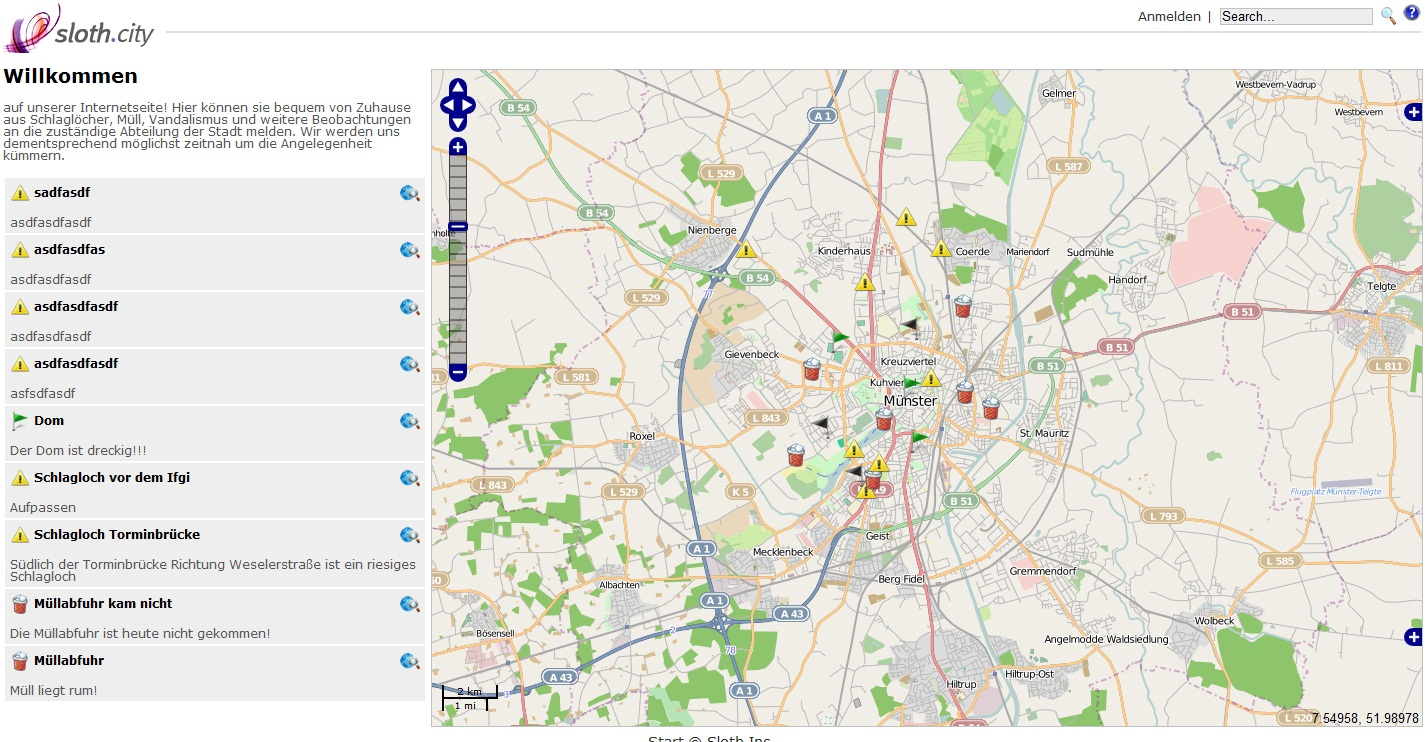
\includegraphics[width = 15 cm]{img/ueberblick}
\caption{Überblick der Webseite}
\label{Überblick}
\end{figure}


Die \textbf{Karte} ist das zentrale Element der Seite sloth.city, da dort ein Überlick über die eingetragenen Beschwerden vorzufinden ist. Die Karteninteraktion erfolgt über die Zoom und Pan Panels. Des Weiteren werden im unteren Bereich der Karte, die jeweiligen Koordinaten angezeigt. Die gesichteten Beobachtungen werden ebenfalls über die Karte hinzugefügt (siehe Beobachtungen anlegen). Der rechte Rand der Karte beinhaltet zwei Menüpunkte. Der obere Menüpunkt lässt die Auswahl zwischen drei Karten. Der untere Menüpunkt hingegen beinhaltet eine Übersichtskarte. 

Im rechten oberen Teil der Seite ist eine \textbf{Anmeldung} möglich oder eine \textbf{Suche} nach den eingetragenen Beobachtungen. Sollten sie Probleme jeglicher Art haben, können sie uns natürlich auch kontaktieren. Die Hilfe Schaltfläche steht ihnen hierfür zur Verfügung.  

Die eingetragenen \textbf{Beobachtungen} werden untereinander auf der linken Seite direkt neben der Karte dargestellt. Jedes Symbol hat ihre eigene Kategorie. Wird eine Beobachtung in der Karte nicht gefunden, kann die Zoom-Funktion benutzt werden.

Im unteren Bereich haben sie mit dem \textbf{Start} Schriftzug die Möglichkeit zurück zur Hauptseite zu gelangen. Diesen Teil werden sie in jeder Ebene dieser Webseite wiederfinden.


\newpage

\section{Besucher}
Wie schon erwähnt gibt es die Möglichkeit mit der Webseite sloth.city als Besucher zu interagieren. Ohne Anmeldung können sie nur einige der Funktionen nutzen. 
Die erwähnten Funktionen im Überblick Abschnitt kann ein Besucher dieser Webseite vollständig ausführen (außer Beobachtungen anlegen!).

\subsection{Beobachtungen}
Die wichtigste Funktion der Webseite ist die Erstellung von Beobachtungen. Normalerweise kann durch Klick in die Karte eine Beobachtung erstellt werden. Ein Fenster öffnet sich und mehrere Optionen stehen zur Verfügung. Diese Möglichkeit kann der Besucher nicht nutzen, da eine Meldung erscheint, dass er sich dafür anmelden muss. 

\begin{figure}[h]
\centering
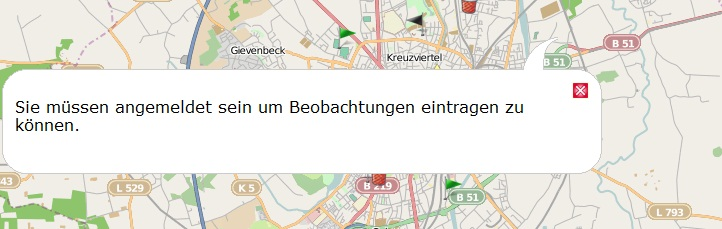
\includegraphics[width = 10 cm]{img/anmelden}
\caption{Anmelden}
\label{Anmelden}
\end{figure}

\subsection{Editieren}
Auch die Möglichkeit Beobachtungen zu editieren, also zu verändern, entfällt komplett. Nur als Administrator oder eingeschränkt als Nutzer kann man Beobachtungen verändern.

\newpage

\section{Administrator}
Als Administrator obliegt einem die Verwaltung der Benutzer, Beobachtungen, Kategorien und Meldungen. Nur der Administrator kann Benutzer löschen, alle Beobachtungen editieren, Kategorien erstellen, editieren, löschen sowie Meldungen editieren und löschen.  

Die Registrierung des Administrators erfolgt über eine Besonderheit. Der erste Benutzer der Webseite ist gleichzeitig auch der Administrator.

\subsection{Verwaltung}
Um in die Verwaltungsebene zu gelangen klicken sie auf ihre angegebene Administrator e-mail Adresse.
\begin{figure}[h]
\centering
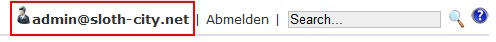
\includegraphics[width = 10 cm]{img/adminemail}
\caption{E-Mail Administrator}
\label{E-Mail Administrator}
\end{figure} 

\subsubsection{Verwaltungsoptionen}
Es gibt 4 Verwaltungsoptionen. Die Benutzerverwaltung, Beobachtungsverwaltung, Kategorieverwaltung und die Meldungsverwaltung.
\begin{figure}[h]
\centering
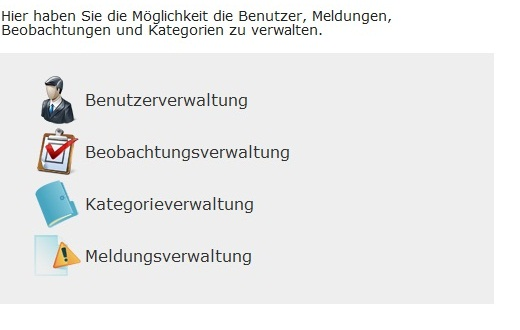
\includegraphics[width = 10 cm]{img/Verwaltung}
\caption{Verwaltung}
\label{Verwaltung}
\end{figure}

\newpage

\subsubsection{Benutzerverwaltung}
In der Benutzerverwaltung können sie als Administrator die jeweiligen Benutzer editieren. Der Nachname, Vorname, die E-mail Adresse, das Passwort oder die Benutzergruppe lassen sich ändern.
\begin{figure}[h]
\centering
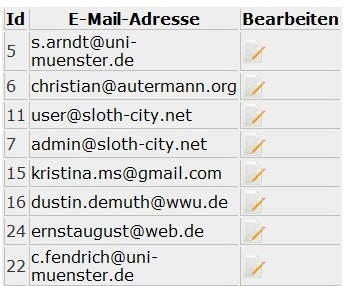
\includegraphics[width = 10 cm]{img/Benutzerverwaltung}
\caption{Benutzerverwaltung}
\label{Benutzerverwaltung}
\end{figure}

\subsubsection{Beobachtungsverwaltung}
Hier lassen sich Beobachtungen editieren, löschen oder neu erstellen.
\begin{figure}[h]
\centering
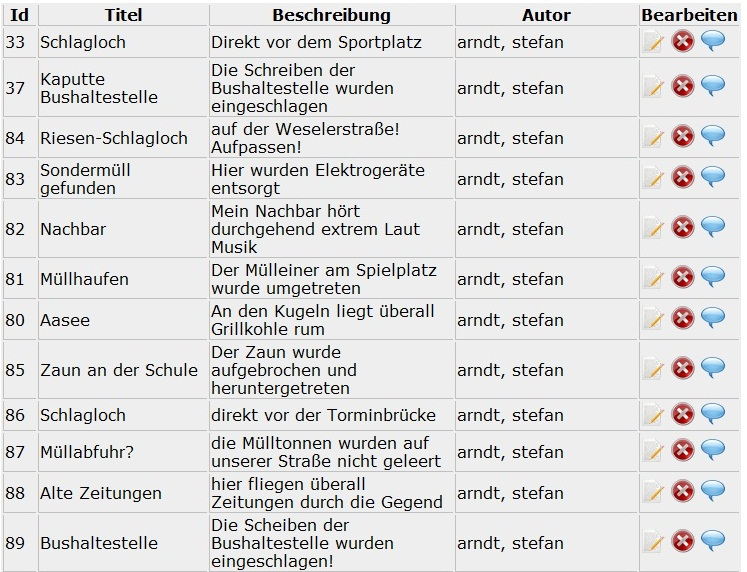
\includegraphics[width = 10 cm]{img/Beobachtungsverwaltung}
\caption{Beobachtungenverwaltung}
\label{Beobachtungenverwaltung}
\end{figure}

\newpage
\subsubsection{Kategorieverwaltung}
Hier lassen sich die Kategorien erstellen, löschen und editieren.
\begin{figure}[h]
\centering
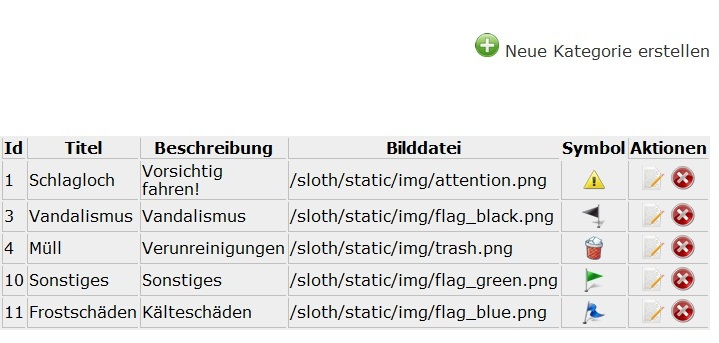
\includegraphics[width = 10 cm]{img/Kategorieverwaltung}
\caption{Kategorieverwaltung}
\label{Kategorieverwaltung}
\end{figure}

\subsubsection{Meldungsverwaltung}
Meldungen lassen sich editieren und löschen. Sollte eine Meldung den Status "`Offen"' haben, kann diese durch die Editierfunktion auf "`Bearbeitet"' gesetzt werden. Hierfür muss lediglich ein Haken hinter Status im Editiermodus gesetzt und durch Submit bestätigt werden. Natürlich kann dies auch wieder rückgängig gemacht werden.
\begin{figure}[h]
\centering
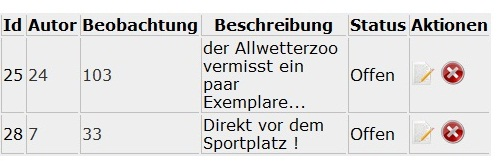
\includegraphics[width = 10 cm]{img/Meldungsverwaltung}
\caption{Meldungsverwaltung}
\label{Meldungsverwaltung}
\end{figure}

\newpage

\section{Benutzer}
Der Benutzer kann Konten löschen, bearbeiten, seine Beobachtungen einsehen und alle Beobachtungen einsehen.
\subsection{Anmelden}
Um sich als Benutzer anzumelden müssen sie sich erst registrieren. Sie klicken auf Anmelden und danach auf Registrieren. Nun muss das Formular ausgefüllt werden.
\begin{figure}[h]
\centering
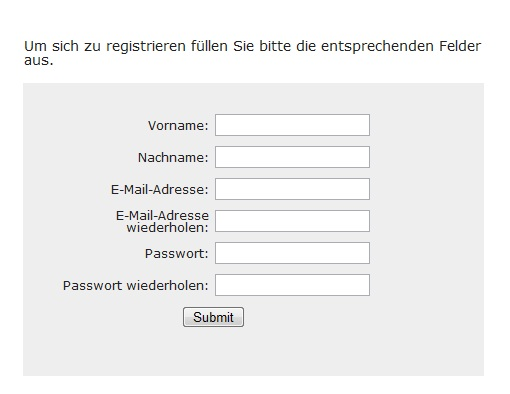
\includegraphics[width = 10 cm]{img/benutzeranmelden}
\caption{Benutzer anmelden}
\label{Benutzer anmelden}
\end{figure}

Sollte das Formular ausgefüllt sein, muss der Prozess mit Submit bestätigt werden.

\subsection{Verwaltung}
Um in die Verwaltungsebene zu gelangen klicken sie auf ihre angegebene Benutzer E-mail Adresse.
\begin{figure}[h]
\centering
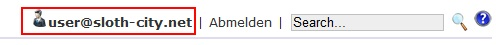
\includegraphics[width = 10 cm]{img/benutzeremail}
\caption{Benutzer e-mail}
\label{Benutzer e-mail}
\end{figure}

\newpage

\subsubsection{Verwaltungsoptionen}
Es gibt vier Verwaltungsoptionen. Sie können ein Konto löschen, bearbeiten, ihre und alle Beobachtungen einsehen.
\begin{figure}[h]
\centering
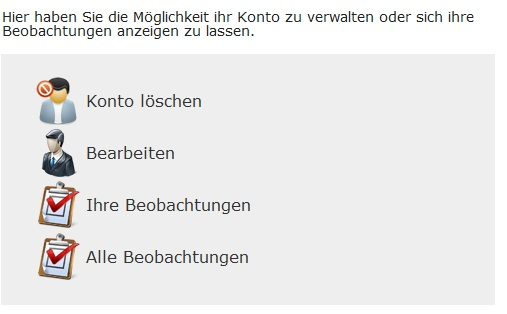
\includegraphics[width = 10 cm]{img/Benutzerverwaltung2}
\caption{Benutzerverwaltung}
\label{Benutzerverwaltung}
\end{figure}

\subsubsection{Konto löschen}
Sie können ihr Konto löschen, indem sie einfach mit Submit bestätigen.
\begin{figure}[h]
\centering
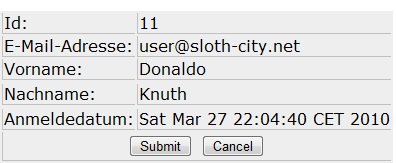
\includegraphics[width = 10 cm]{img/kontoloeschen}
\caption{Konto löschen}
\label{kontoloeschen}
\end{figure}

\newpage

\subsubsection{Konto bearbeiten}
Sie können ihr Konto bearbeiten und dann mit Update bestätigen.
\begin{figure}[h]
\centering
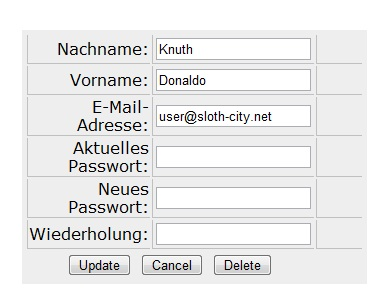
\includegraphics[width = 10 cm]{img/kontobearbeiten}
\caption{Konto bearbeiten}
\label{kontobearbeiten}
\end{figure}

\subsubsection{Ihre Beobachtungen}
Sie können ihre Beobachtungen bearbeiten, löschen und eine neue Meldung hinzufügen.
\begin{figure}[h]
\centering
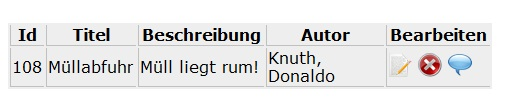
\includegraphics[width = 10 cm]{img/ihrebeobachtungen}
\caption{Ihre Beobachtungen}
\label{Ihre Beobachtungen}
\end{figure}

\subsubsection{Alle Beobachtungen}
Sie können alle Beobachtungen einsehen.
\begin{figure}[h]
\centering
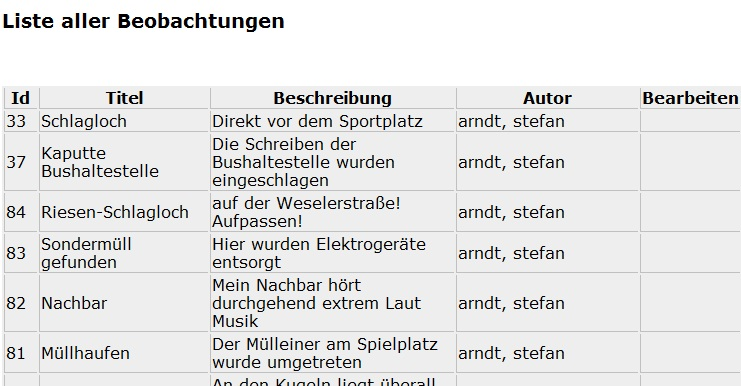
\includegraphics[width = 10 cm]{img/allebeobachtungen}
\caption{Alle Beobachtungen}
\label{Alle Beobachtungen}
\end{figure}


\newpage


\section{Beobachtungen anlegen}
Beobachtungen anzulegen ist ein wesentlicher Bestandteil der Webseite. Wenn sie einen Problemfall in einer Gegend festgestellt haben, dann können sie per Klick in die Karte eine neue Beobachtung anlegen. Beobachtungen können sie als Administrator und als registrierter Nutzer anlegen.
\begin{figure}[h]
\centering
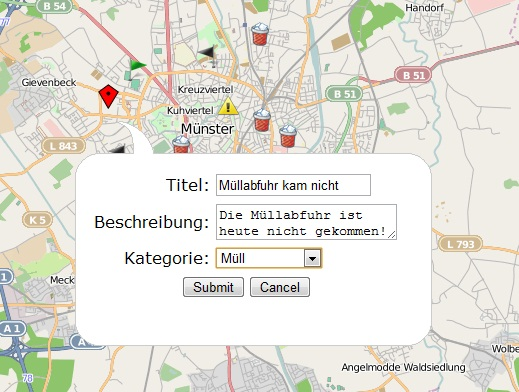
\includegraphics[width = 10 cm]{img/beobachtunganlegen}
\caption{Beobachtung anlegen}
\label{Beobachtung anlegen}
\end{figure}

Wenn sie die Beobachtung wie im Beispiel ausgefüllt haben, können sie diese mit Submit bestätigen. Ihre neu angelegte Beobachtung wird in der Beobachtungsliste links von der Karte angezeigt.
\begin{figure}[h]
\centering
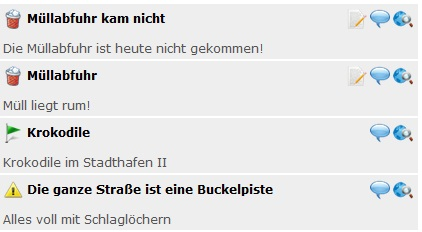
\includegraphics[width = 10 cm]{img/beobachtungsliste}
\caption{Beobachtungen}
\label{Beobachtungsliste}
\end{figure}


\newpage

\section{Kontakt}
Sollten sie Probleme mit dem Handbuch oder der Webseite haben können sie uns unter der folgenden Adresse kontaktieren.
\\[1em]
\begin{center}
Support Informationen
\end{center}
\begin{table}[h]
\begin{center}
{\footnotesize
\begin{tabular}{|p{0.2\textwidth}|p{0.25\textwidth}|p{0.25\textwidth}|p{0.25\textwidth}|}

\hline
									
						Name & Sloth Support  									\\\hline
						Straße, Hausnummer  & Sloth Allee, -1    \\\hline
						Stadt, PLZ &  Virtual City, 42   					\\\hline
						Webseite  & www.vespuccis.de   						 \\\hline
						E-Mail  & sloth@vespuccis.de   							\\\hline
						Telefon   & support.contact.phone     			 \\\hline
						Telefax &  	 support.contact.fax 						  \\\hline
					

\end{tabular}
}

\end{center}
\end{table}


\end{document}



